\documentclass[11pt]{article}
\usepackage[utf8]{inputenc}
\usepackage[T1]{fontenc}
\usepackage{graphicx}
\usepackage{longtable}
\usepackage{wrapfig}
\usepackage{rotating}
\usepackage[normalem]{ulem}
\usepackage{amsmath}
\usepackage{amssymb}
\usepackage{capt-of}
\usepackage{hyperref}
\usepackage[danish, ]{babel}
\usepackage[margin=2.5cm]{geometry}
\usepackage{lmodern}
\usepackage[style=verbose-ibid,backend=bibtex]{biblatex}
\usepackage{csquotes}
\usepackage{comment}
\usepackage{float}
\usepackage{parskip}
\usepackage{fancyhdr}
\usepackage{setspace}
\onehalfspacing
% Appendix, attachments management
\usepackage[toc,page]{appendix} %
\renewcommand{\appendixtocname}{Appendiks}
\renewcommand{\appendixpagename}{\centering{Appendiks}}
\usepackage{pdfpages} % Including PDF-pages
    \usepackage{eso-pic}
    \usepackage{atbegshi}
    \usepackage{ifthen}
    \usepackage{calc}
\addbibresource{bibliography.bib}
\hypersetup{colorlinks, linkcolor=blue, urlcolor=blue}
\author{Rasmus Elias Sandkær \& Jeppe Bøgeskov Bech}
\date{\today}
\title{Eksamensprojekt}
\hypersetup{
pdfauthor={Rasmus Elias Sandkær \& Jeppe Bøgeskov Bech},
pdftitle={Eksamensprojekt},
pdfkeywords={},
pdfsubject={},
pdfcreator={Emacs 29.4 (Org mode 9.7.11)}, 
pdflang={Danish}}

%% Start af dokumentet
\begin{document}
    %% Forside
    \newgeometry{top=2.0cm, bottom=2.0cm}
\begin{titlepage}
    \centering

    \vspace*{1cm}

    % Title and subtitle are enclosed between two rules.
    \rule{\textwidth}{1pt}

    % Title
    \vspace{.7\baselineskip}
    {\huge \textbf{Projekt 3 - Eksamensprojekt}}

    % Subtitle
    \vspace*{.5cm}
    {\LARGE Forårssemester 2025}

    \rule{\textwidth}{1pt}

    \vspace{1cm}

    % Set this size for the remaining titlepage.
    \large

    % Authors side by side, using two minipages as a trick.

    \begin{table}[h]
        \centering
        \begin{tabular}{cc}
            \begin{minipage}{.5\textwidth}
                \centering
                Jeppe Bøgeskov Bech \\
                {\normalsize \url{jepp9920@zbc.dk}}
            \end{minipage}
            &
            \begin{minipage}{.5\textwidth}
                \centering
                Rasmus Elias Sandkær \\
                {\normalsize \url{rasm999v@zbc.dk}}
            \end{minipage}
        \end{tabular}
    \end{table}








    % More authors can be inserted here with additional minipages.

    \vspace{1cm}

    % Report logo.
    % \fbox{\includegraphics[width=.7\textwidth]{./assets/forsidebillede.png}}

    \vfill

    % University and date information at the bottom of the titlepage.
    2. x \\
    ZBC Handels- og Teknisk gymnasium Slagelse \\
    Akademisk år 2024-2025 \\
    \today
\end{titlepage}

    \restoregeometry
    \tableofcontents
    \newpage

    %% Indledning
    \section{Indledning}
    \subsection{Projektstyring}


    %% Problemformulering
    \section{Problemformulering}
    Problemformulering
Vi lever i et højere teknologisk samfund, hvor mange af os benytter teknologi på daglige basis, men I nutidens tilfælde af krig er der rigtigt stor risiko for hacker angreb, som ikke bare svækker militære styrker, men også vores allesammen hverdag.
Det leder os frem til følgende overordnede spørgsmål, vi vil besvare i rapporten:

•	Hvad er årsagerne til, og konsekvenserne af, teknologiske angreb under krig - og hvad kan vi gøre ved det?

For at kunne besvare dette spørgsmål, må vi først undersøge følgende:

Her stiller i spørgsmål der relaterer til problemtræet
\begin{itemize}
    \item Hvordan skal vi kunne gøre kommunikation nemmere under en krig
    \item Hvad skal man kunne gøre i tilfælde af blackout
    \item Hvordan skal man ku tilkalde hjælp og backup under krig
    \item Hvordan skal samfundet hænge sammen forhold til de teknologiske blackouts.
\end{itemize}

Ovenstående spørgsmål vil blive besvaret i problemanalysen
Problemanalyse

Årsagerne til teknologiske angreb under krig
En af de største årsager til teknologiske angreb under krig er den stigende afhængighed af teknologi i militære operationer.
herefter kan de også måle deres angreb mod civil infrastruktur. som gir fjenden muligheden for, at målrette deres angreb mod kritisk infrastruktur og kommunikationssystemer. konsekvenserne kan være, at Hospitaler og redningskøretøjer ikke kan kommunikere med hinanden, som vil resultere at civile mennesker med kritiske tilstande ikke kan få hjælp i tide.
ikke vil kunne få hjælp i tide. og herefter også folk som er hospitaliseret som har brug for højere teknologiske værktøjer til at kunne overleve, heller ikke vil være istand til at få hjælp. kommunikation mellem lægerne vil også miste effektivitet, grunden manglen på kommunikation mellem hospital sektioner.


    
    %% Problemanalyse
    \section{Problemanalyse}
    Det følgende afsnit vil indeholde en omfattende besvarelse af spørgsmålene som ses i problemformuleringen.

\subsection{Spørgsmål A}
I dette afsnit vil vi besvare spørgsmålet: ``Hvordan kan vi gøre nødstilfælde nemmere at håndtere ?''

Her tager vi fat i en HV-model, som er en model til at finde ud af, hvordan man kan håndtere problemet.

\begin{table}[H]
    \centering
    \begin{tabular}{|p{4cm}|p{10cm}|}
        \hline
        1. Hvad? &
        \begin{itemize}
            \item Hvad skal man gøre, når man har brug for nødhjælp?
            \item Hvad bliver gjort, i nødstilfælde?
            \item Hvad burde blive gjort, under nødstilfælde?
            \item Hvad kan ellers gøres, i et nødstilfælde?
            \item Hvad burde ellers blive gjort, i et nødstilfælde?

        \end{itemize} \\
        \hline
        2. Hvorfor? &
        \begin{itemize}
            \item Hvorfor gør han/hun det at kalde efter nødhjælp?
            \item Hvorfor ringe efter nødhjælp?
            \item Hvorfor gør man det på den måde at man skal fortage et opkald?
        \end{itemize} \\
        \hline
        3. Hvem? &
        \begin{itemize}
            \item Hvem ringer efter nødhjælp?
            \item Hvem burde ringe efter nødhjælp?
            \item Hvem kan ellers ringe efter nødhjælp?
        \end{itemize} \\
        \hline
        4. Hvor? &
        \begin{itemize}
            \item Hvor skal man ringe efter nødhjælp?
            \item Hvor bliver det behandlet, i en krisesituation?
            \item Hvor burde det blive gjort, at ringe efter nødhjælp?
        \end{itemize} \\
        \hline
        5. Hvornår? &
        \begin{itemize}
            \item Hvornår skal man gøre det?
            \item Hvornår bliver det gjort?
            \item Hvornår burde det blive gjort?
        \end{itemize} \\
        \hline
        6. Hvordan? &
        \begin{itemize}
            \item Hvordan gør man det?
            \item Hvordan bliver det gjort?
            \item Hvordan burde det blive gjort?
            \item Er der en anden måde at gøre det på?
        \end{itemize} \\
        \hline
    \end{tabular}
    \caption{HV-model til analyse af nødstilfælde under krig.}
    \label{tab:hv-model}
\end{table}

\subsubsection{Beskrivelse af HV-modellen}
\begin{enumerate}
    \item Hvad? \\
    %% I dætte tilfælde kommer vores app til at besvare alle de usikkerheder der kan opstå i en krisessituation.
    I en krisesituation er det afgørende at kunne handle hurtigt og ikke mindst korrekt. Derfor ville en app være en god løsning til at hjælpe danskerne med at håndtere usikkerheder som eventuelt kunne opstå i en krisesituation, og tage borgeren i hånde og herved guide dem igennem processen.

    Appen giver borgeren helt klare og professionelle instruktioner om, ham/hun skal håndtere nødssituationer. Den vigtigste handling er at rinnge 1-1-2, og appen guider vrugeren gennem opkaldet, så den nødvendige information bliver vidregivet til den relavante myndighed. Dette sparer værdigfuld tid i krisesituation, da der kan være et utal af mennesker som fortager opkald til alarmcentralen i tilfælde af f.eks. en naturkatastrofe.
    
    Alt afhængig af situationen, kan der være forskellige handlinger som skal tages. beredskabsstyrelsen har lavet en række anbefalinger på hvordan den almene borger bør forberede sig på eventuelle krier, heri denne vejledning findes seks "beredskabstips" som er følgende: "Kend til 1-1-2", "Kend nærområdets udfordringer", "Vid, hvordan du får information", "Sørg for, at du kan tilkalde hjælp", "Vær kildekritisk" og "Tænk over dine særlige behov". \footfullcite{DuerEndelafberedskabet} Disse anbefalinger bruger vi senere til at lave vores app. \ref{produktprincip}

    Derudover bør man også sikre området - Undgå yderligere fare for dig selv eller andre (f.eks. trafik, brand, gaslækage). under situationen - Hvad er sket? Hvor mange er berørt? Hvilken type hjælp er nødvendig? Yd førstehjælp - Hvis du er i stand til det, og det er sikkert, så giv livreddende førstehjælp (f.eks. hjertemassage, stands blødning).\footfullcite{DanskFørstehjælp}
    
    \item Hvorfor? \\
    I de fleste tilfælde er det en naturlig reaktion at ringe til 1-1-2 hvis man er i nød. Dette kan være fordi man står i en farlig situation, som man ikke selv kan håndtere grundet mangel på viden eller er i fare for at skade sig selv eller mangel på de nødvendige ressourcer til at håndtere situationen. Der kan også være en psykologisk grund til at ringe til 1-1-2, som er at man ikke er i stand til at håndtere situationen, og derfor har brug for hjælp.

    det er den hurtigste måde at få hjælp på, og det er den mest effektive måde at få hjælp på. og på nuverende tidspunkt er der ikke gode apps som kan hjælpe mens man venter på hjælp, især hvis alarmcentralen ikke kan nås, eller de ikke har tid til at guide over telefonen.
    
    \item Hvem? \\
    Oftest er det den anden part, som ikke selv er udsat i situationen, så det er vigtigt for personmen at vide hvordan de skal takle situationen. Og herfor vil en app være en god løsning til at hjælpe borgeren med at håndtere nødssituationer.

    Vedkommende som fortager opkaldet til 1-1-2, afhænger af den konkrete situation, men oftest er det den person som ankommer til ulykkestedet først. Dog anbefales det at følge Dansk Førstehjælpsråds anbefalinger til hvordan man skal yde førstehjælp og hvordan man skal håndtere situationen. \footfullcite{DanskFørstehjælp}

    Alle med en mobiltelefon kan ringe efter nødhjælp i Danmark selv uden et simkort, dette skyldes at 112 er en del af EU's sikkerhedsnetværk. Som dikterer at alle med en mobiltelefon kan ringe efter nødhjælp i Europa. \footfullcite{EENA}


    \item Hvor? \\
    Opkaldet til 1-1-2 skal foretages på stedet, hvor den pågældende ulykke er sket. De vigtigste punkter når opkaldet fortages er at det skal ske fra et sikkert sted, så ulykken ikke forværres, og at der gives præcise oplysninger om situationen her er det vigtigt aldrig at fortælle noget som du tror er sandt, men hvis du ikke er sikker på det.

    Den akutte behandling vil oftest ske på stedet, og hvis det er en større ulykke så bliver det behandlet på et hospital.

    \item Hvornår? \\
    Når du finder person som har brug for hjælp, eller hvis du selv er i nød så skal et opkald til alarmcentralen foretages hurtigst muligt fordi der kan være en stor risiko for at personen ikke kan vente.
    I risikosituationer er det vigtigt at reagere hurtigt og ikke mindst korrekt, når du ringer 1-1-2 så kan du forvente der går 5-20 minutter før ambulancen ankommer, og da en person som ikke trækker vejret kan være i fare for at dø, eller bliver permanent hjerneskadet ("Hjernen kan overleve meget kort tid uden ilt, uden at man får hjerneskade. Efter 4-5 minutters hjertestop, vil manhave svær hjerneskade hvis ikke der udøves hjertelungeredning.")\footfullcite{netdoktorHS} er det vigtigt at du ved hvad du skal gøre indtil hjælpen kommer. \\
    \vspace{1em}
    \item Hvordan? \\
    Førstehjælp udføres jf. Dansk Førstehjælpsråd ved at følge disse 4 hovedpunkter \footfullcite{DanskFørstehjælp}:

    \begin{itemize}
        \item Sikre området:
        Sørg for, at det er sikkert at hjælpe personen. Undgå yderligere fare for dig selv eller andre, som f.eks. trafik, brand eller gaslækage.

        \item Vurdér personen:
        Tjek om personen er ved bevidsthed. Spørg højt: "Er du okay?" Hvis der ikke er nogen reaktion, skal du kontrollere vejrtrækningen.

        \item Tilkald hjælp:
        Ring 1-1-2 og giv præcise oplysninger om situationen, herunder hvad der er sket, hvor det er sket, og hvor mange der er berørt.

        \item Giv førstehjælp:
        Jf. Dansk Førstehjælpsråd, udføres førstehjælpen ved at benytte sig af et af førstehjælpens huskeord M-ABC, hvilket er den rækkefølge førstehjælperen skal udføre den konkrete førstehjælp i. Disse betyder hhv. Massive bleeding, Airway, Breathing og Circulation; og er opstat således at det vigtigste er lægst mod venstre, og vigtigheden daler mod højre.\footfullcite{DanskFørstehjælp}
    \end{itemize}

    Disse trin kan redde liv og hjælpe med at stabilisere en person, indtil professionel hjælp når frem.


\end{enumerate}
\subsection{Spørgsmål B}
Spørgsmålet fra problemformuleringen, som vi vil besvare i dette afsnit, er: ``Spørgsmål 2''.

Vores spørgeskemaundersøgelse viste, at\ldots


\subsection{Miljøovervejelser}

\begin{enumerate}
    \item Energieffektivitet \\
    App'en skal være optimeret til lavt batteriforbrug, da den bruges i nødsituationer, hvor strøm kan være begrænset.
    Push-notifikationer og GPS-tracking skal kun aktiveres ved behov da den ikke skal  køre konstant i baggrunden.
    Begræns datalagring til det nødvendige, og slet automatisk inaktive eller unødvendige data.

    \item Hardwarekompatibilitet \\
    Appen bør understøtte ældre telefonmodeller for at forbedre deres levetid og mindske behovet for udskiftning.

    \item Datatransport og netværksforbrug \\
    Minimer datamængden appen sender og modtager, primært områder med lav netdækning
\end{enumerate}

\subsection{Brug af empiri}
Vi har benyttet os af den kvantitative til at udarbejdet et spørgeskema, som 50 personer har besvaret. Spørgsmålene omhandlede nødsituationer, hvor der kan være behov for akut hjælp.\\
Det første spørgsmål lød:\\
\textbf{"Har du været ude for en nødsituation, der krævede øjeblikkelig hjælp – enten som vidne til eller deltager i en hændelse, f.eks. hjertestop?"}\\
Her svarede 39 \% ja. Dette er særligt interessant, da ca. 4 ud af 5 danskere har lært førstehjælp. Det betyder, at cirka 8 \% af dem, der har oplevet en nødsituation, ikke har haft kompetencerne til at yde førstehjælp – hvilket kan få fatale konsekvenser.\footfullcite{beredskabsinfo} \\
Dernæst spurgte vi, om deltagerne tidligere har ringet 1-1-2. Kun 26,3 \% svarede ja. Ser vi på de 8 \% uden førstehjælpsviden og krydser det med dem, der ikke har ringet 1-1-2, ender vi med, at omtrent 2 \% af alle, der har været i en nødsituation, hverken har kunnet yde førstehjælp eller tilkaldt hjælp. Statistisk set svarer det til, at ud af 1000 personer i en akut situation vil omkring 20 risikere at stå uden nogen form for hjælp – hvilket potentielt kan være livstruende.\\
Vi har også spurgt, om folk har brugt SOS-funktionen på deres telefon. Hele 91,9 \% svarede nej. 
Det vil sige af de 26,1 \%, som har ringet 1-1-2, har kun 8,1 \% anvendt telefonens indbyggede \textbf{SOS-funktion}. Det svarer til cirka 2,08 \% af det samlede antal, der har kontaktet alarmcentralen – altså en meget lav udnyttelse af en funktion, der ellers er bredt tilgængelig i moderne smartphones.\\
Vil vil nu gå i dybden med det i konkurrentanalysen:


    %% Bibliografi
    \newpage
    \printbibliography[heading=bibintoc,title={Litteraturliste}]

    %% Appendiks
    \newpage
    \begin{appendices}\newpage
        \renewcommand{\thesubsection}{\Alph{subsection}}
        \subsection{Projektbeskrivelse \label{apx:projektbeskrivels}} \newpage
        \renewcommand*{\thepage}{A\arabic{page}}
        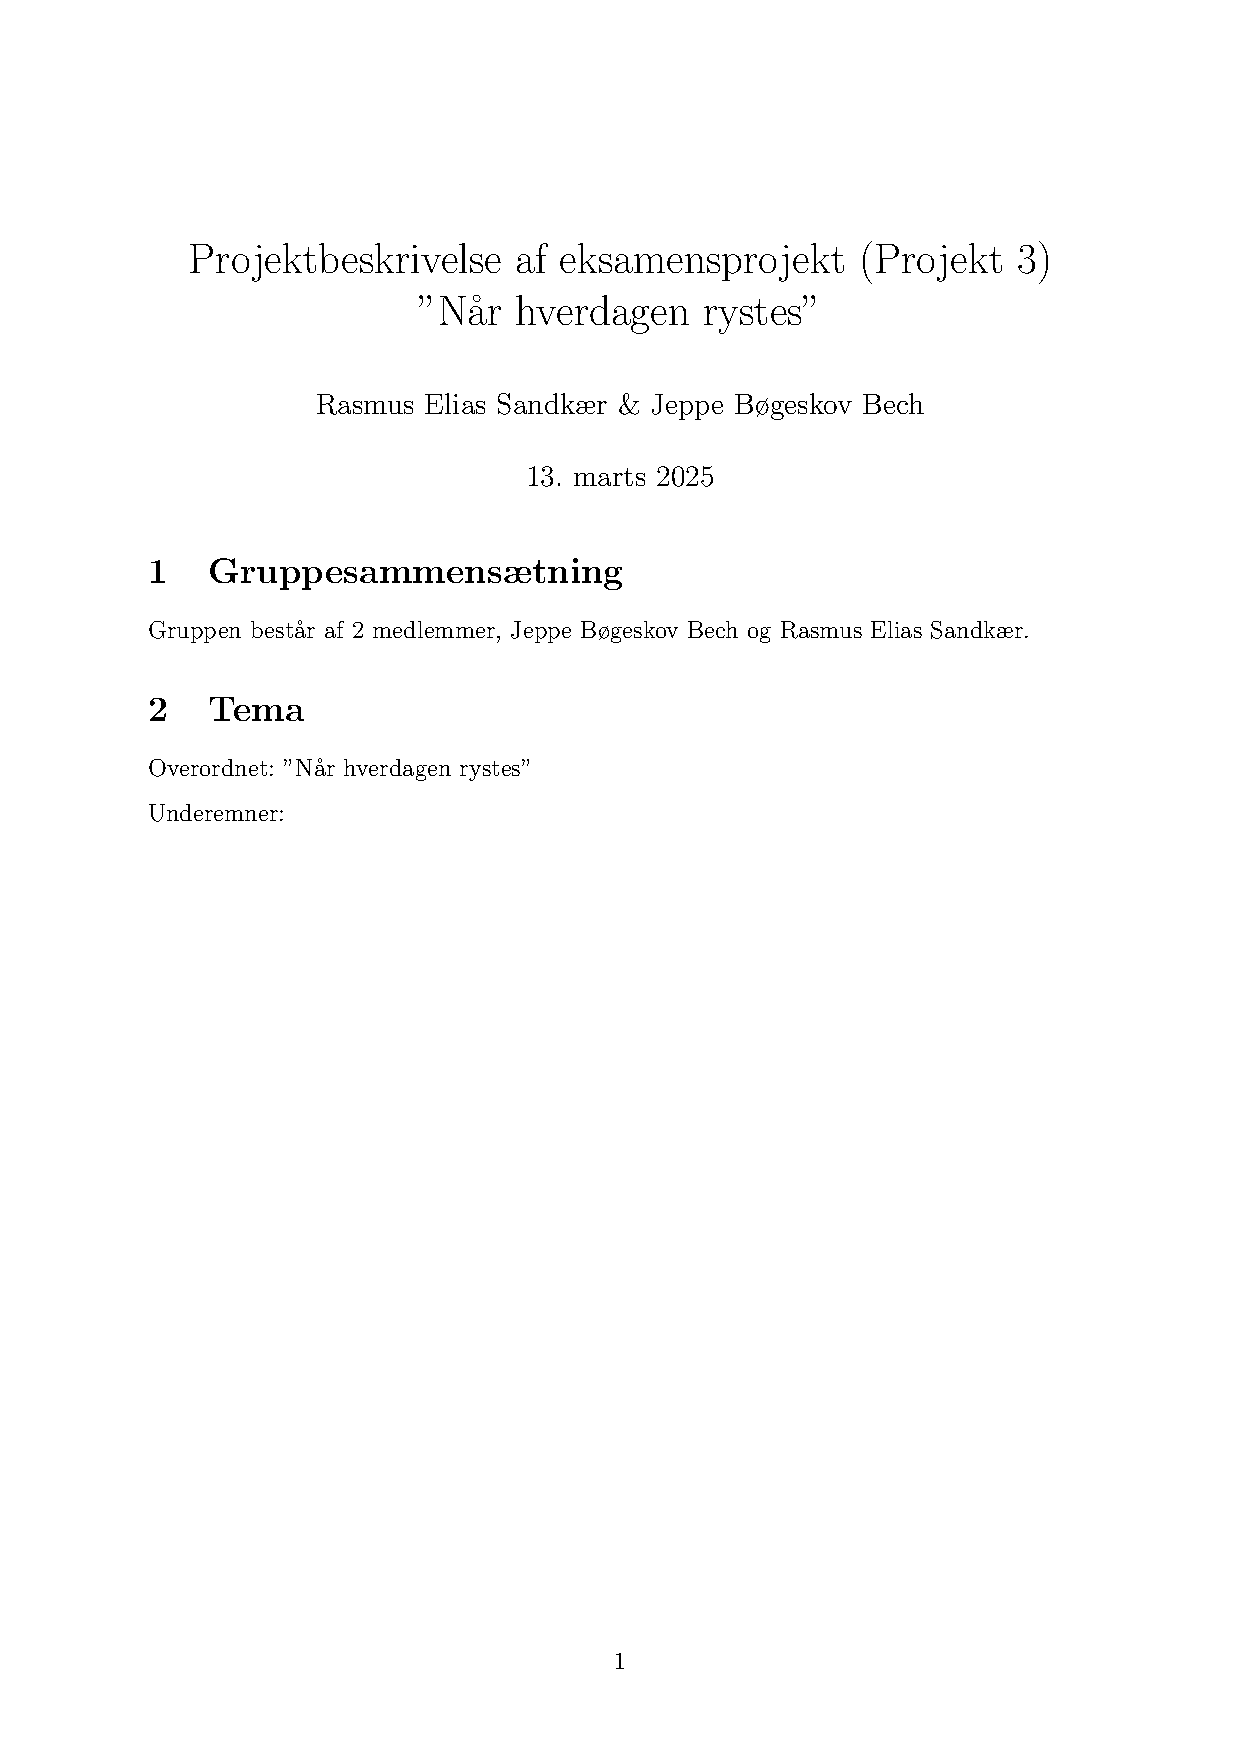
\includepdf[pages=-,delta=5 5,frame=true,landscape=false,nup=1x1,pagecommand={\thispagestyle{plain}}]{./projektbeskrivelse.pdf}
    \end{appendices}
\end{document}
